\documentclass{article}
\usepackage[margin=1in]{geometry}
\usepackage{hyperref}
\usepackage{pdfpages}
\usepackage{siunitx}
\title{Annotated Bibliography}
\author{Adam Newton Wright}
  \date{\today}
\begin{document}
\maketitle

%%%%%%%%%%%%%%%%%%%%%%%%%%%%%%%%%%%%%%%%%%%%%%%%%%
% LambdaChrome Laser Dyes
%%%%%%%%%%%%%%%%%%%%%%%%%%%%%%%%%%%%%%%%%%%%%%%%%%
\section*{Brackman, Ulrick, ``Lambdachrome Laser Dyes,” Lambda Physik 3, (2000)}
This paper is a reference paper rather than a source. It extensively details various laser dyes, at which wavelengths they lase, the range of wavelength they emit at, peak wavelengths, concentrations, solvents, and their efficiencies. It also describes the chemical structure of the dye, physical appearance, and molar absorptivity.

This paper is relevant for determining which dye is appropriate for converting $532 \si{\nano \meter}$ light into the correct wavelength for absorption spectroscopy of sodium or rubidium. It also helps us in preparing the dyes and checking if our efficiency lines up with their predicted efficiency.

\section*{Budker, Dmitry, and Romalis, Michael. ``Optical Magnetometry.” Nature Physics 3, (2007).}
This paper details atomic magnetometry, which is the process of measuring the magnetic field by interacting near resonant light with atoms. Since magnetic fields split the energy levels within the atom and, for atoms with a magnetic moment, requires the atoms precess in what is known as Larmor precession, the absorption profile of the atom. Thus, by measuring the amount of light transmitted through an atomic medium while varying the wavelength of incident light, the magnetic field can be measured with sensitivity. 

This paper is relevant as it describes the theory and application of an experiment similar to mine. Although we are not looking to measure the magnetic field locally, we are looking to see how the absorption of an atom changes with magnetic field. It will be useful for my theory and experiment sections.
%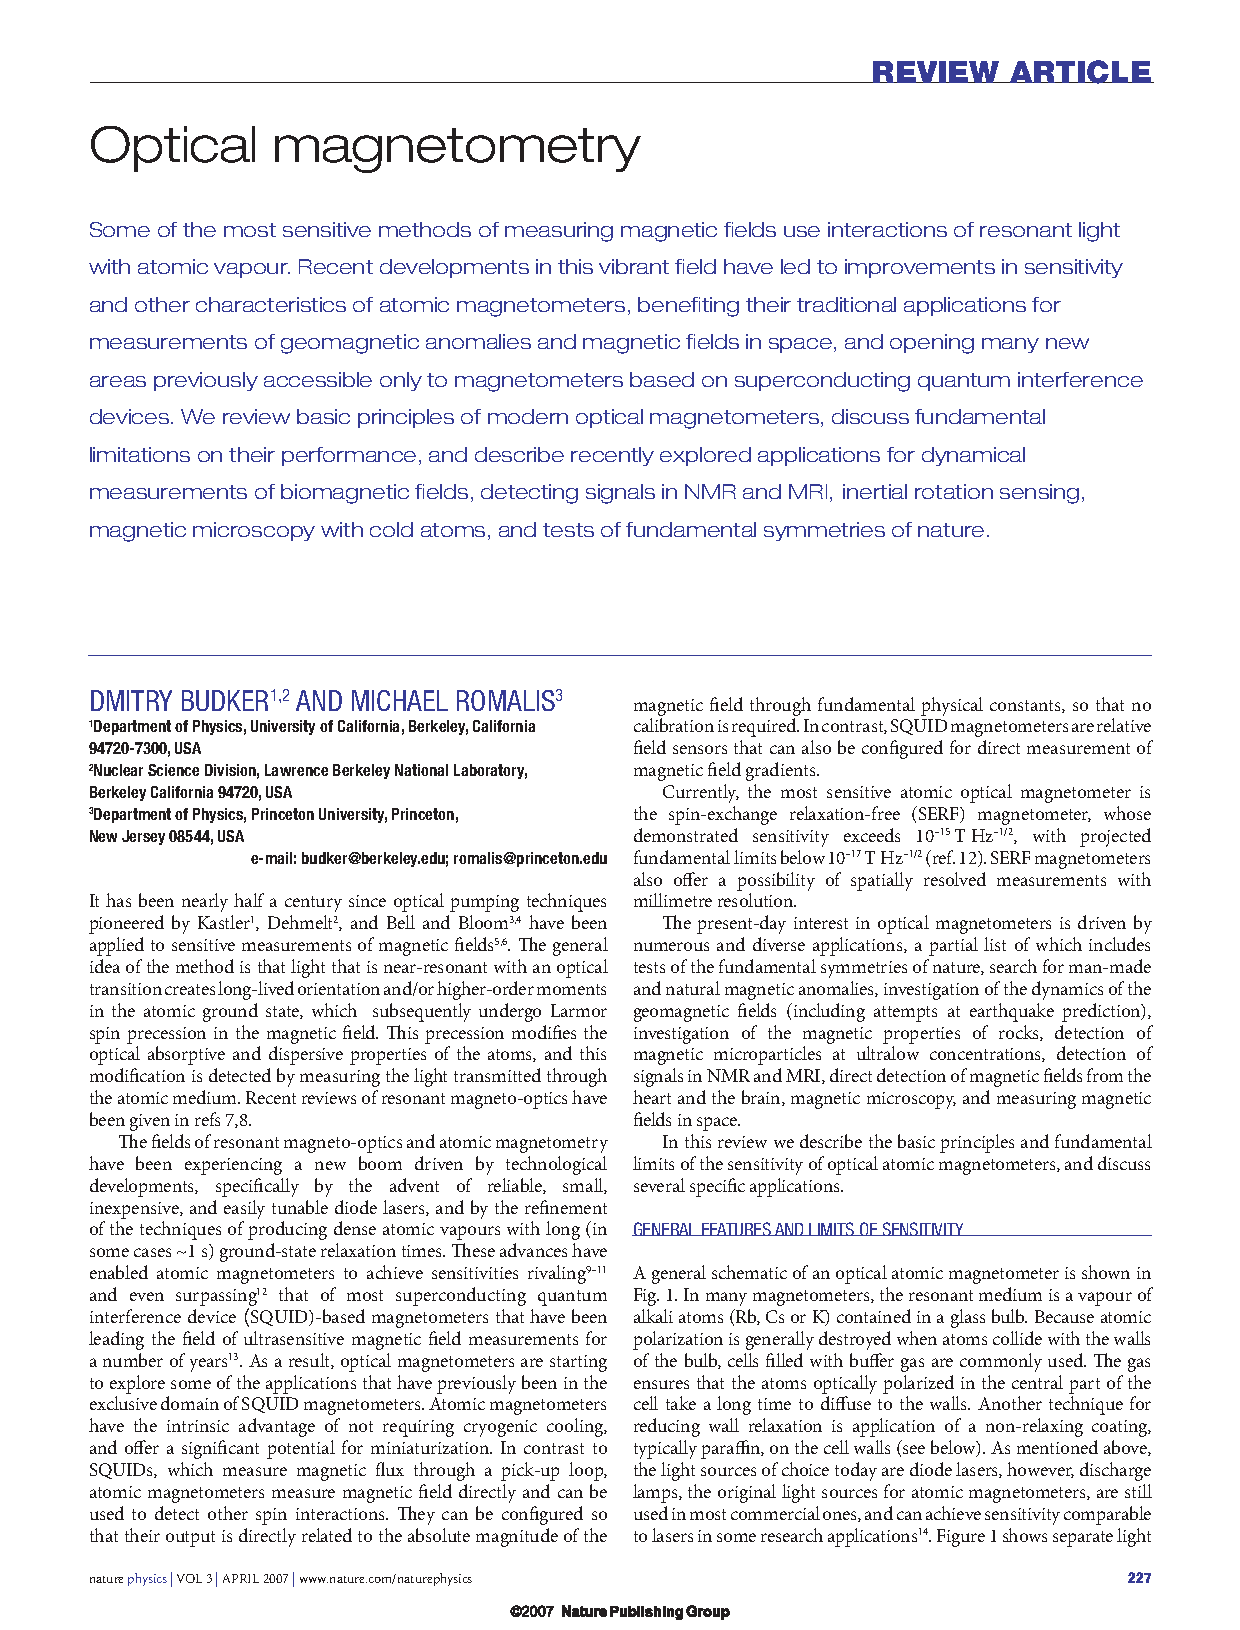
\includepdf[pages =-]{PDF/Optical_magnetometry.pdf}


\section*{Fan, Tingwei, Tianhua Zhou, and Yan Feng. ``Improving sodium laser guide star brightness by polarization switching." Scientific reports 6, (2016).}
This paper states that pumping an optical medium with light that switches between right and left circular polarized light is proposed to improve efficiency. They run numerical simulations which show that this is indeed true, and give the optimal frequency of polarization switching.

This paper is a nice comparison to our experiment, as it provides a theoretical and numerical background for a similar experiment. The only difference is that they use switching of polarization while we will use pulsed laser light in order to match the Larmor frequency.

%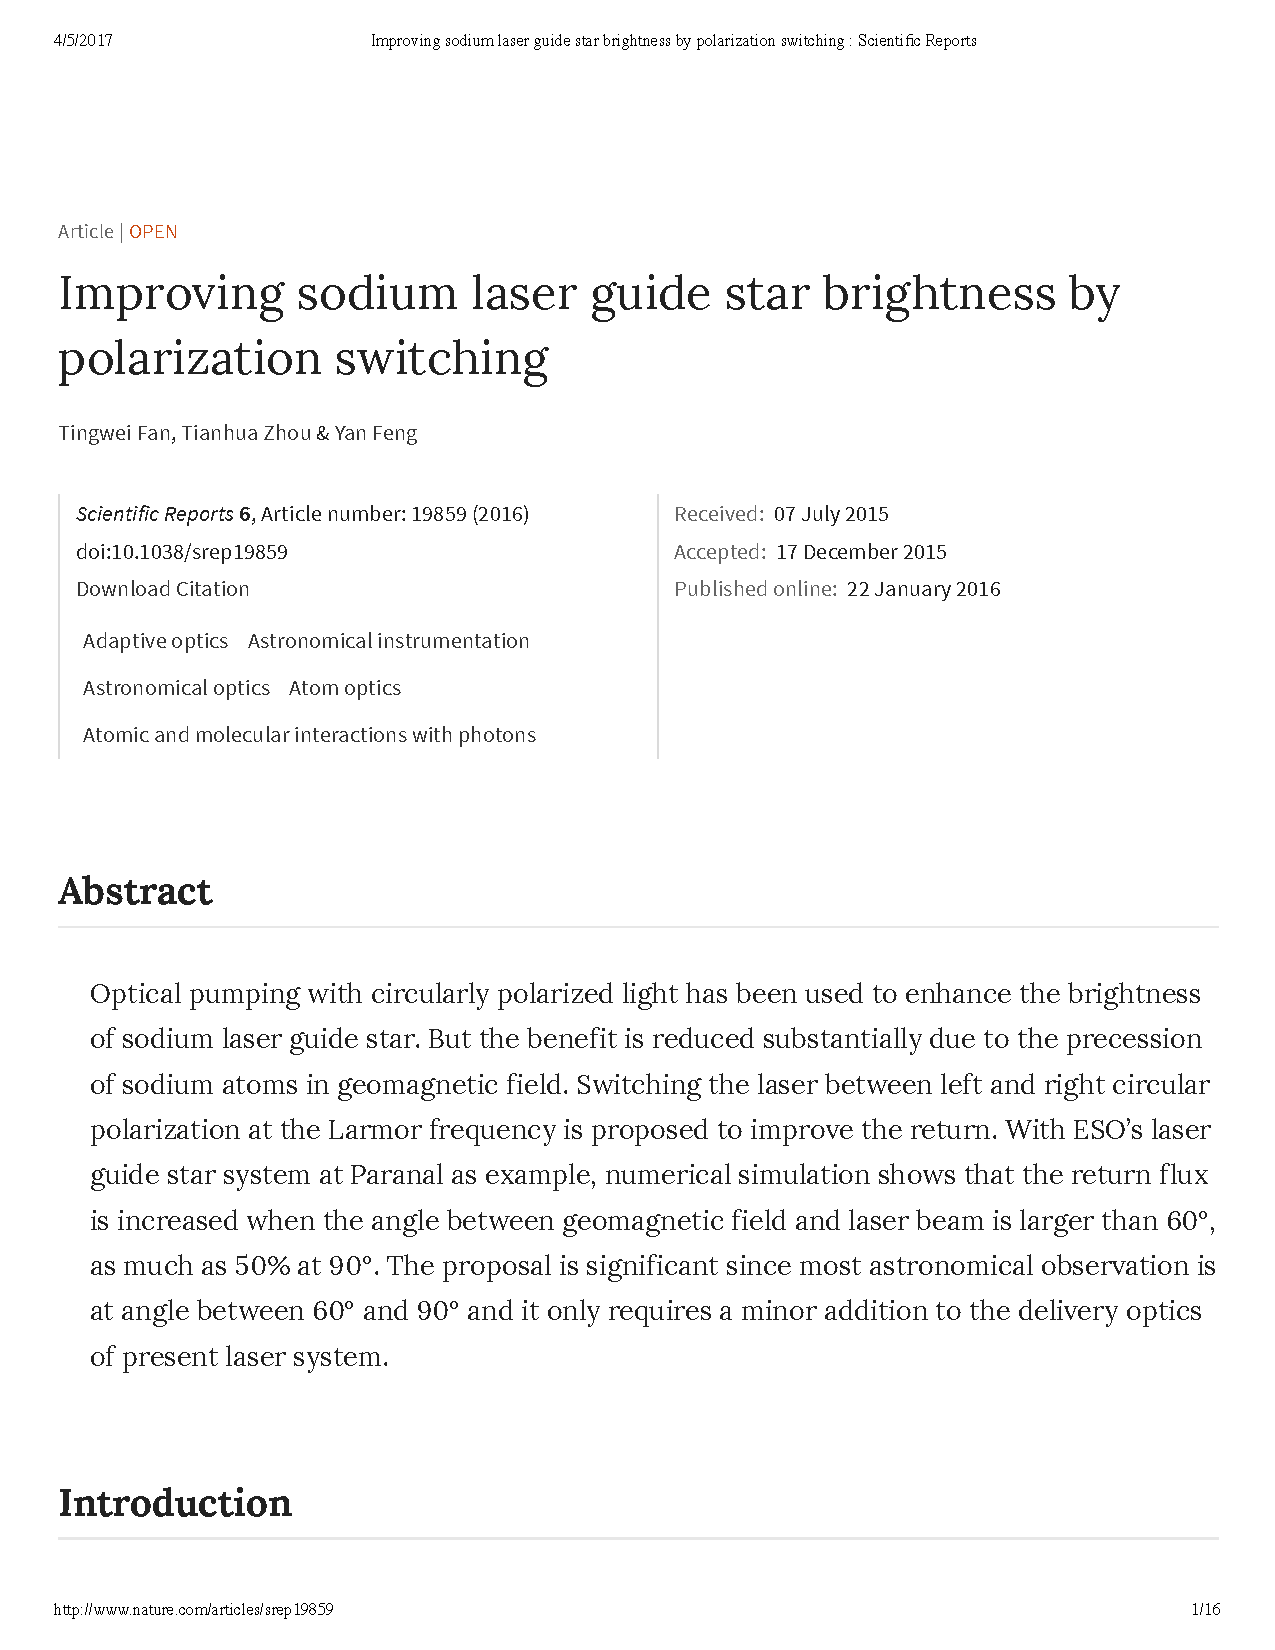
\includepdf[pages=-]{PDF/Improving_lgs_brightness_polarization_switching}

\section*{Fugate, Robert Q., and D. L. Fried. ``Measurement of atmospheric wavefront distortion using scattered light from a laser guide-star." Nature 353.6340, (1991)}
This paper describes how wavefront detection and measurement works in regards to laser guide star systems. 

This paper is not directly related to our experiment, but is relevant to one application of our results, and is worth knowing in general.

%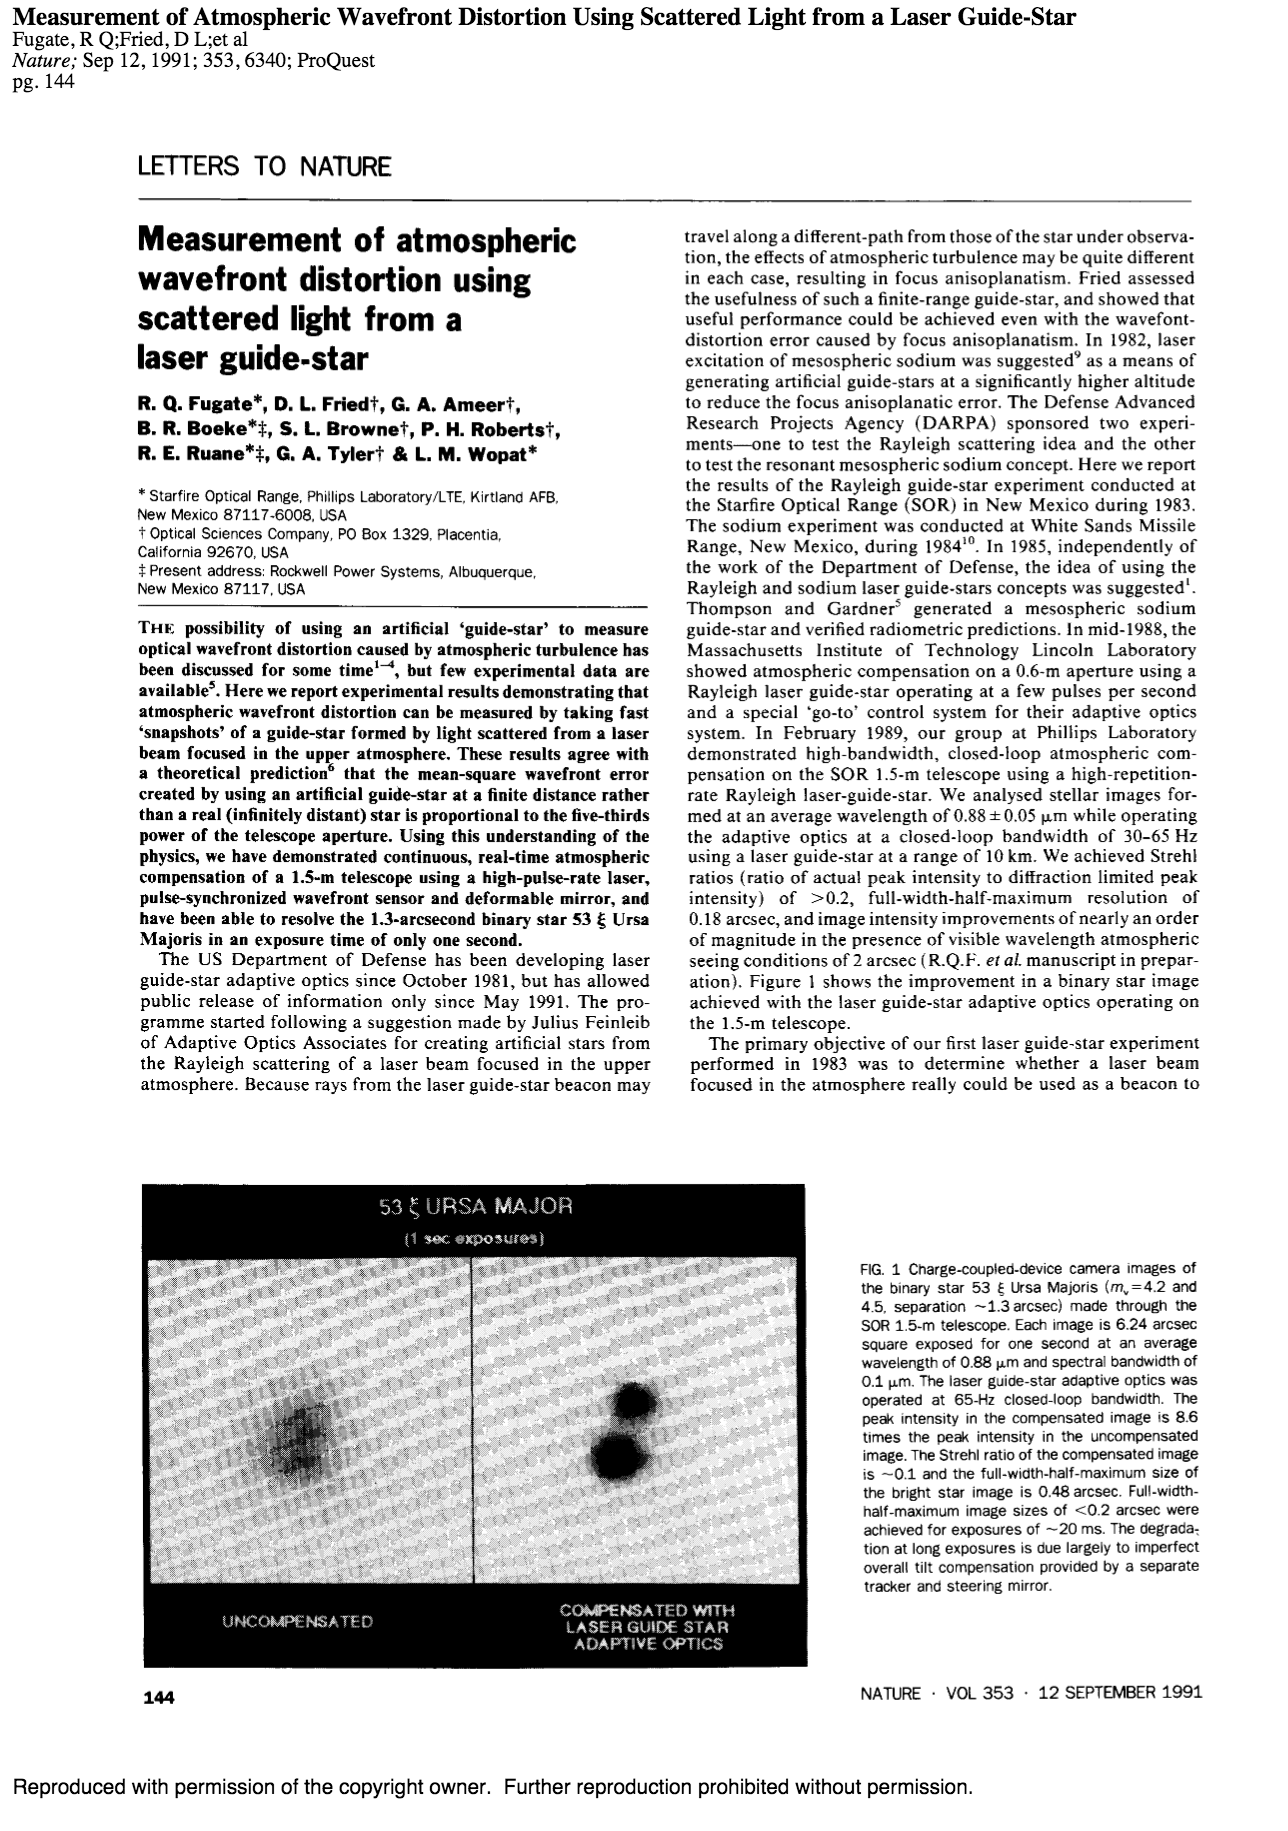
\includepdf[pages=-]{PDF/measurement_atmospheric_distortion.pdf}

\section*{Gale, G. M., B. Pedersen, and P. Schanne. ``Kilohertz picosecond distributed-feedback dye laser system." Optics Communications 76.2, 138-142 (1990).}
A light paper on a kilohertz picosecond dye laser.
This paper describes one possible configuration of a kilohertz-picosecond dye laser. It uses a 65 ps, 1kHz pump laser at 532 nm. This pump is quite similar to our pump, so it should be possible to use their dye laser configuration.

This is quite relevant as we are not quite sure how we are going to configure the dye laser system. It need to be relatively small due to the pulse length of light we are dealing with (i.e. light needs to oscillate back and forth in the cavity several times during the pulse length in order for gain to occur).

%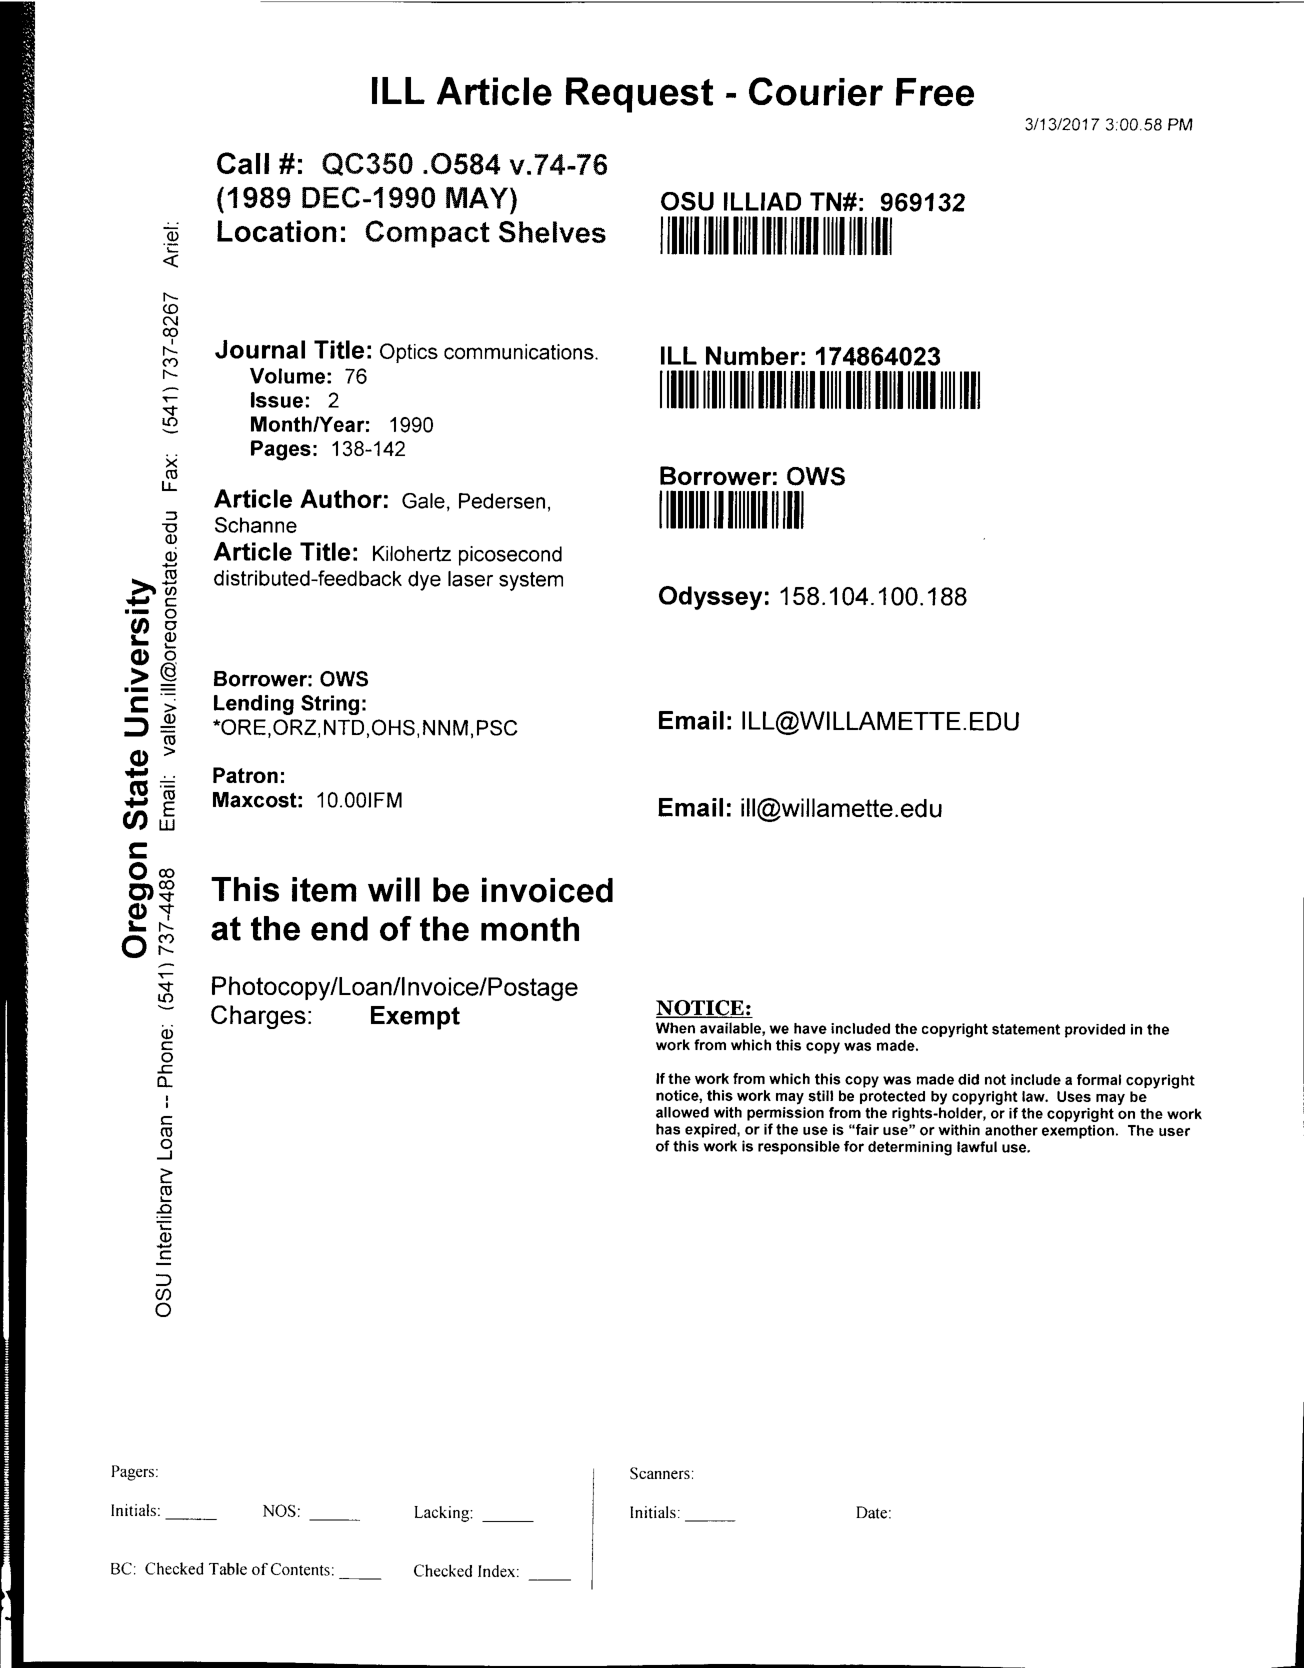
\includepdf[pages=-]{PDF/kilohertz_picosecond_dyelaser.pdf}

\section*{Kane, Thomas J., Paul D. Hillman, and Craig A. Denman. "Pulsed laser architecture for enhancing backscatter from sodium." SPIE Astronomical Telescopes+ Instrumentation. International Society for Optics and Photonics, (2014).}

This paper is awesome, and is more or less the foundation of this experiment. It describes magnetic resonant pulsing, which is the optical pumping of an atomic medium in a magnetic field at a repetition rate equal to that of the Larmor frequency. It describes the theory of this process, as well as numerical simulations for sodium in the geomagnetic field.

%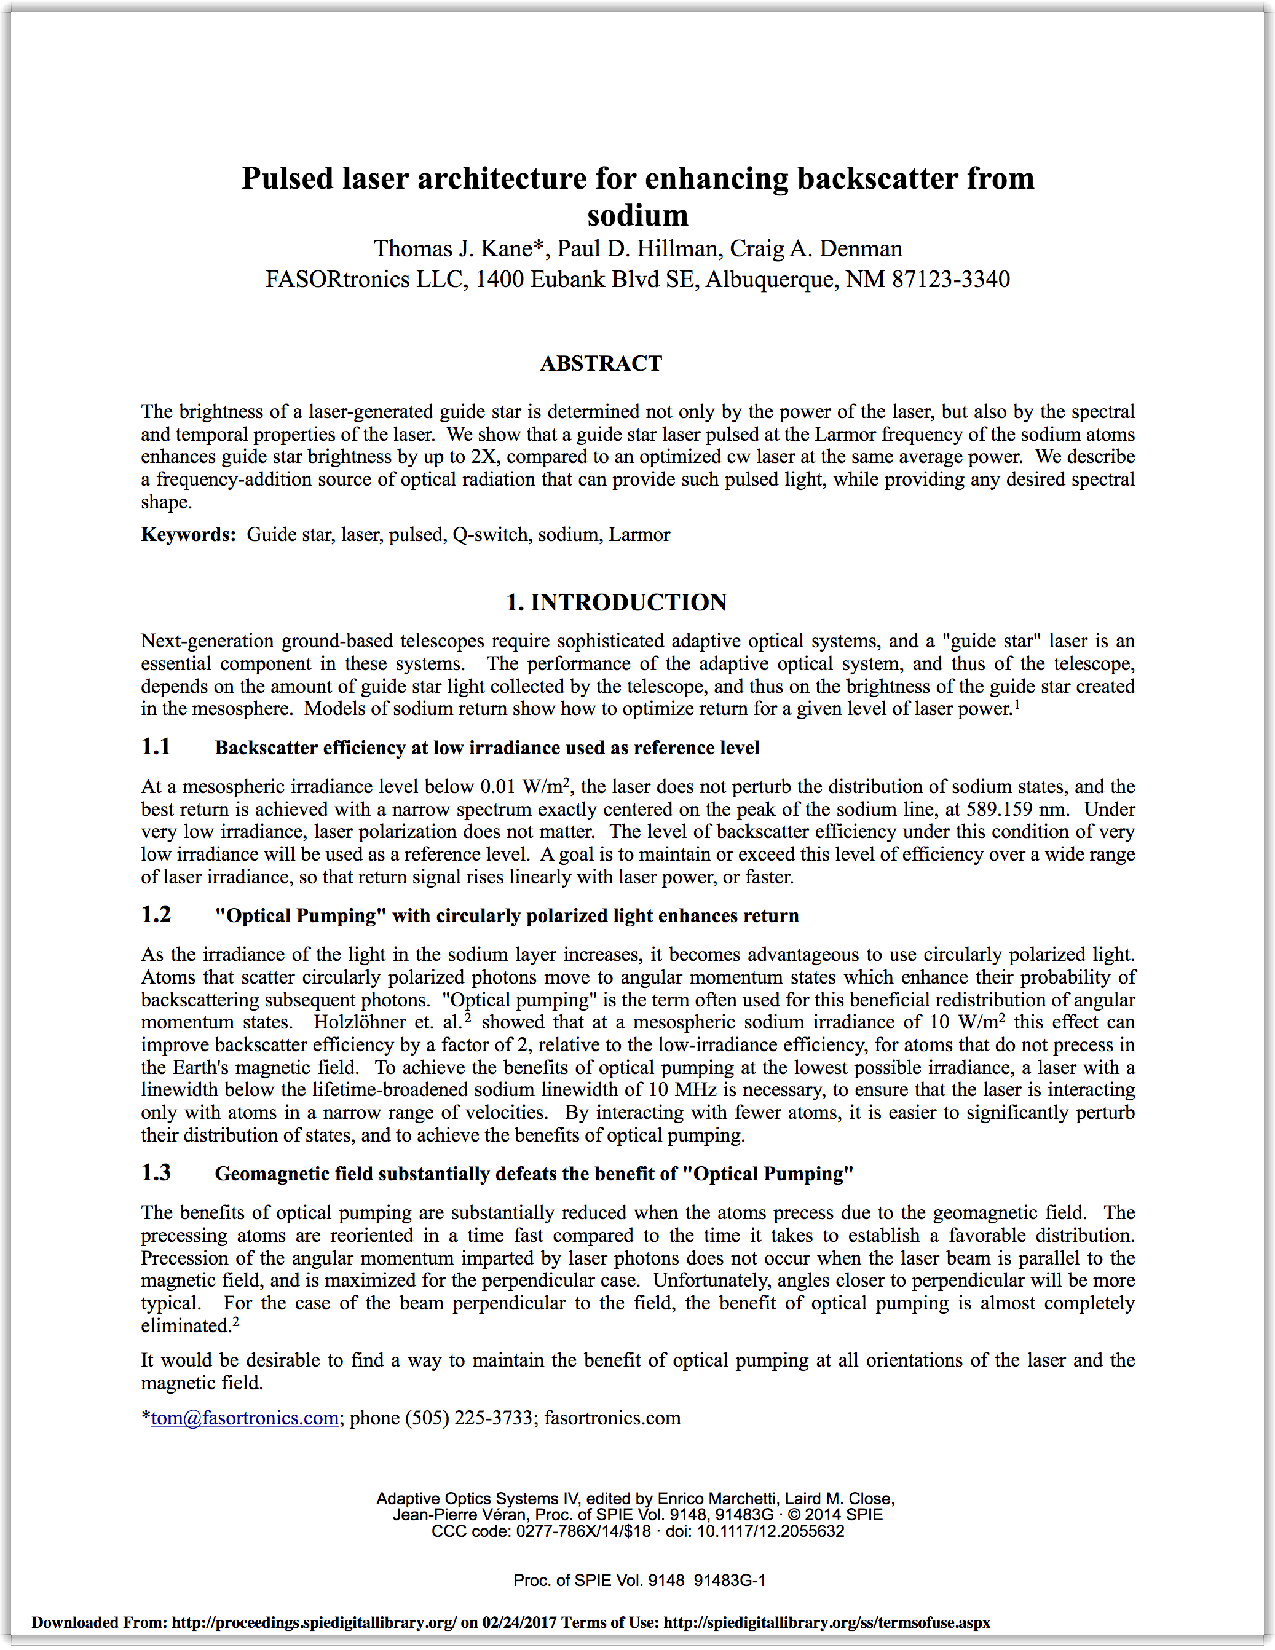
\includepdf[pages=-]{PDF/Pulsed_laser_architecture.pdf}


\section*{Kibblewhite, Edward. "The physics of the sodium laser guide star: Predicting and enhancing the photon returns." In Advanced Maui Optical and Space Surveilance Technologies Conference, (2009).}

This is a great paper detailing the theory of optical pumping and the theory behind laser guide stars. It digs into the quantum/atomic theory of sodium absorption, including a good description of optical pumping. Its theory is concerned primarily with CW lasers, but also proposes how chirping and pulsed lasers could increase photon return.

This paper is relevant as it gives a good theoretical background on how optical pumping works, and what is going to quantum mechanically. This will be great for the background/theory section of my paper.


%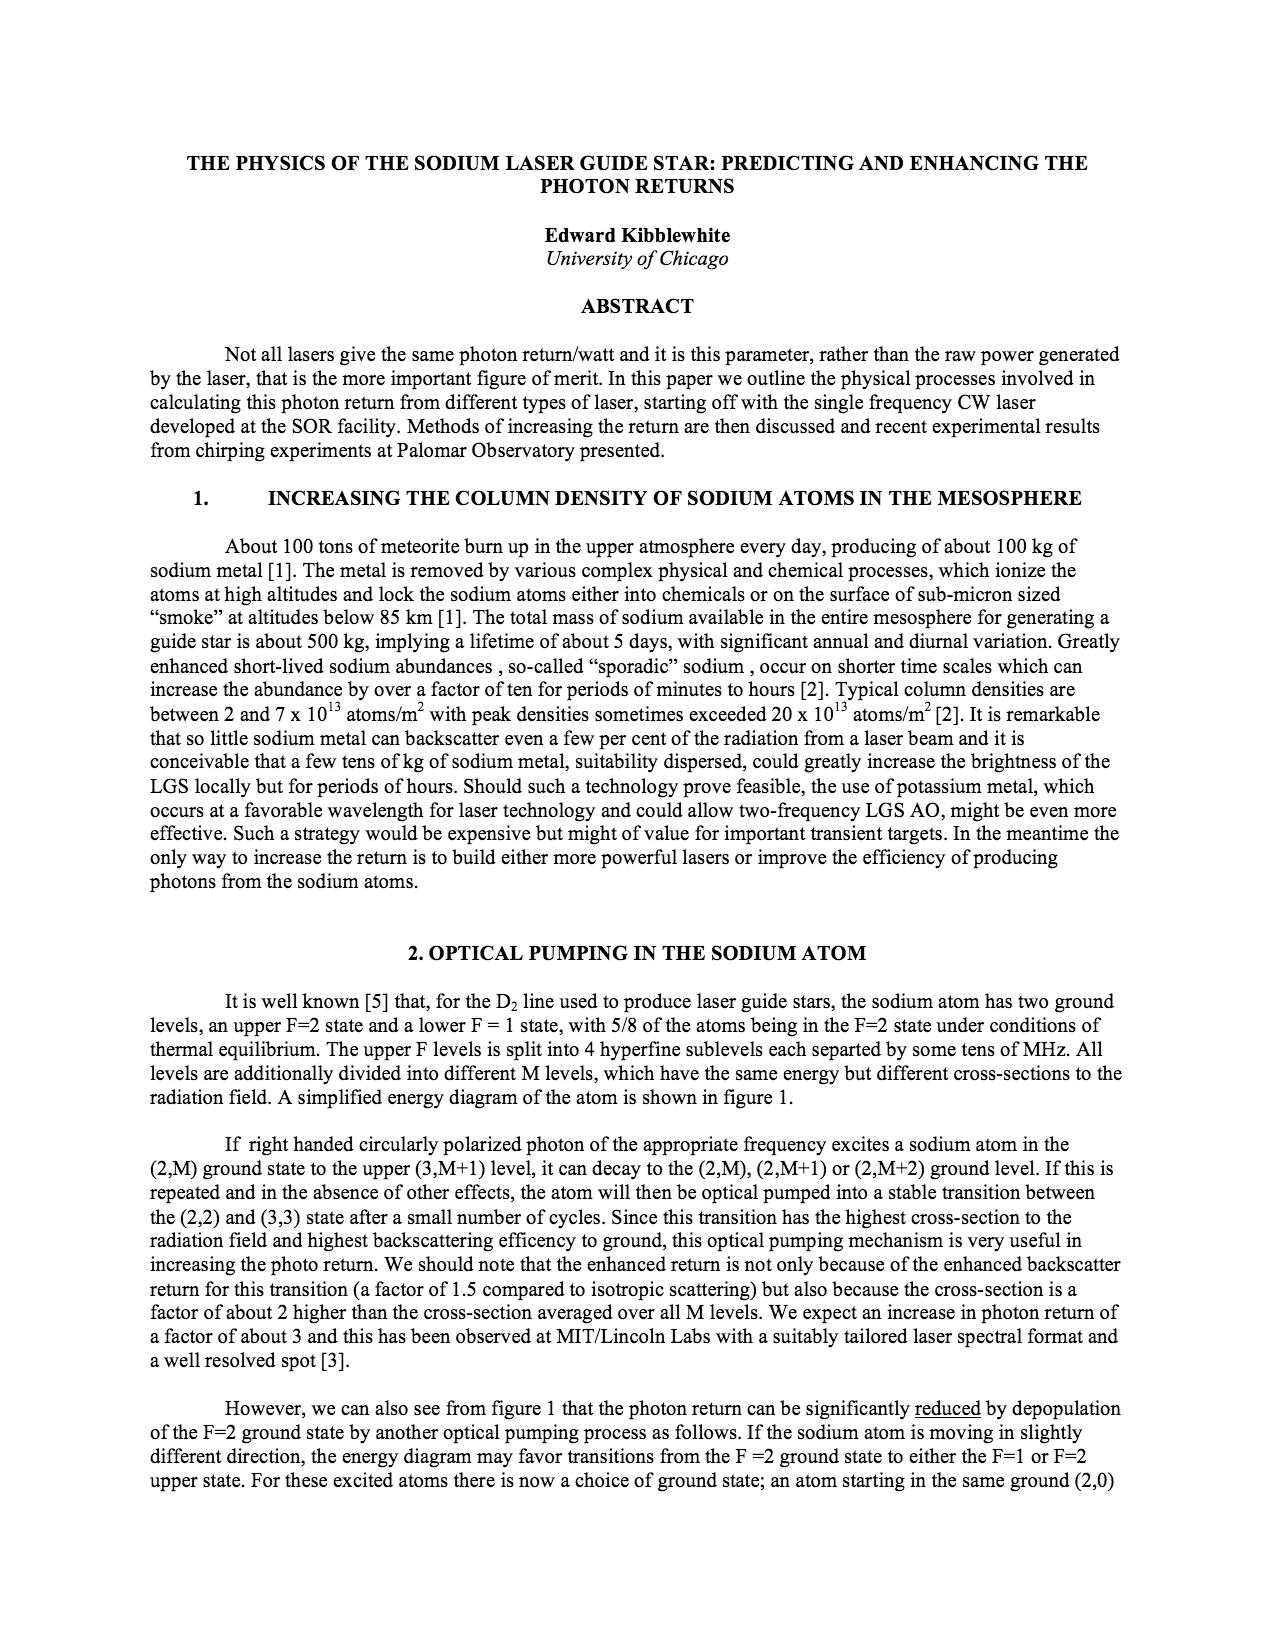
\includepdf[pages = -]{PDF/physics_of_sodium_lgs.pdf}

\section*{Rampy, Rachel, Donald Gavel, Simon M. Rochester, and Ronald Holzlöhner. "Toward optimization of pulsed sodium laser guide stars." JOSA B 32, 12,  2425-2434 (2012).}

This paper is where I originally learned about magnetic resonant pulsing in order to increase photon return of laser guide stars. It compares CW LGS systems to pulsed LGS systems, and also describes how the magnetic field orientation affects the photon return (in a simplified way).

It is relevant as it gives a good introduction to MRP, and gives some numerical simulations that back the claim the MRP will increase photon return.

%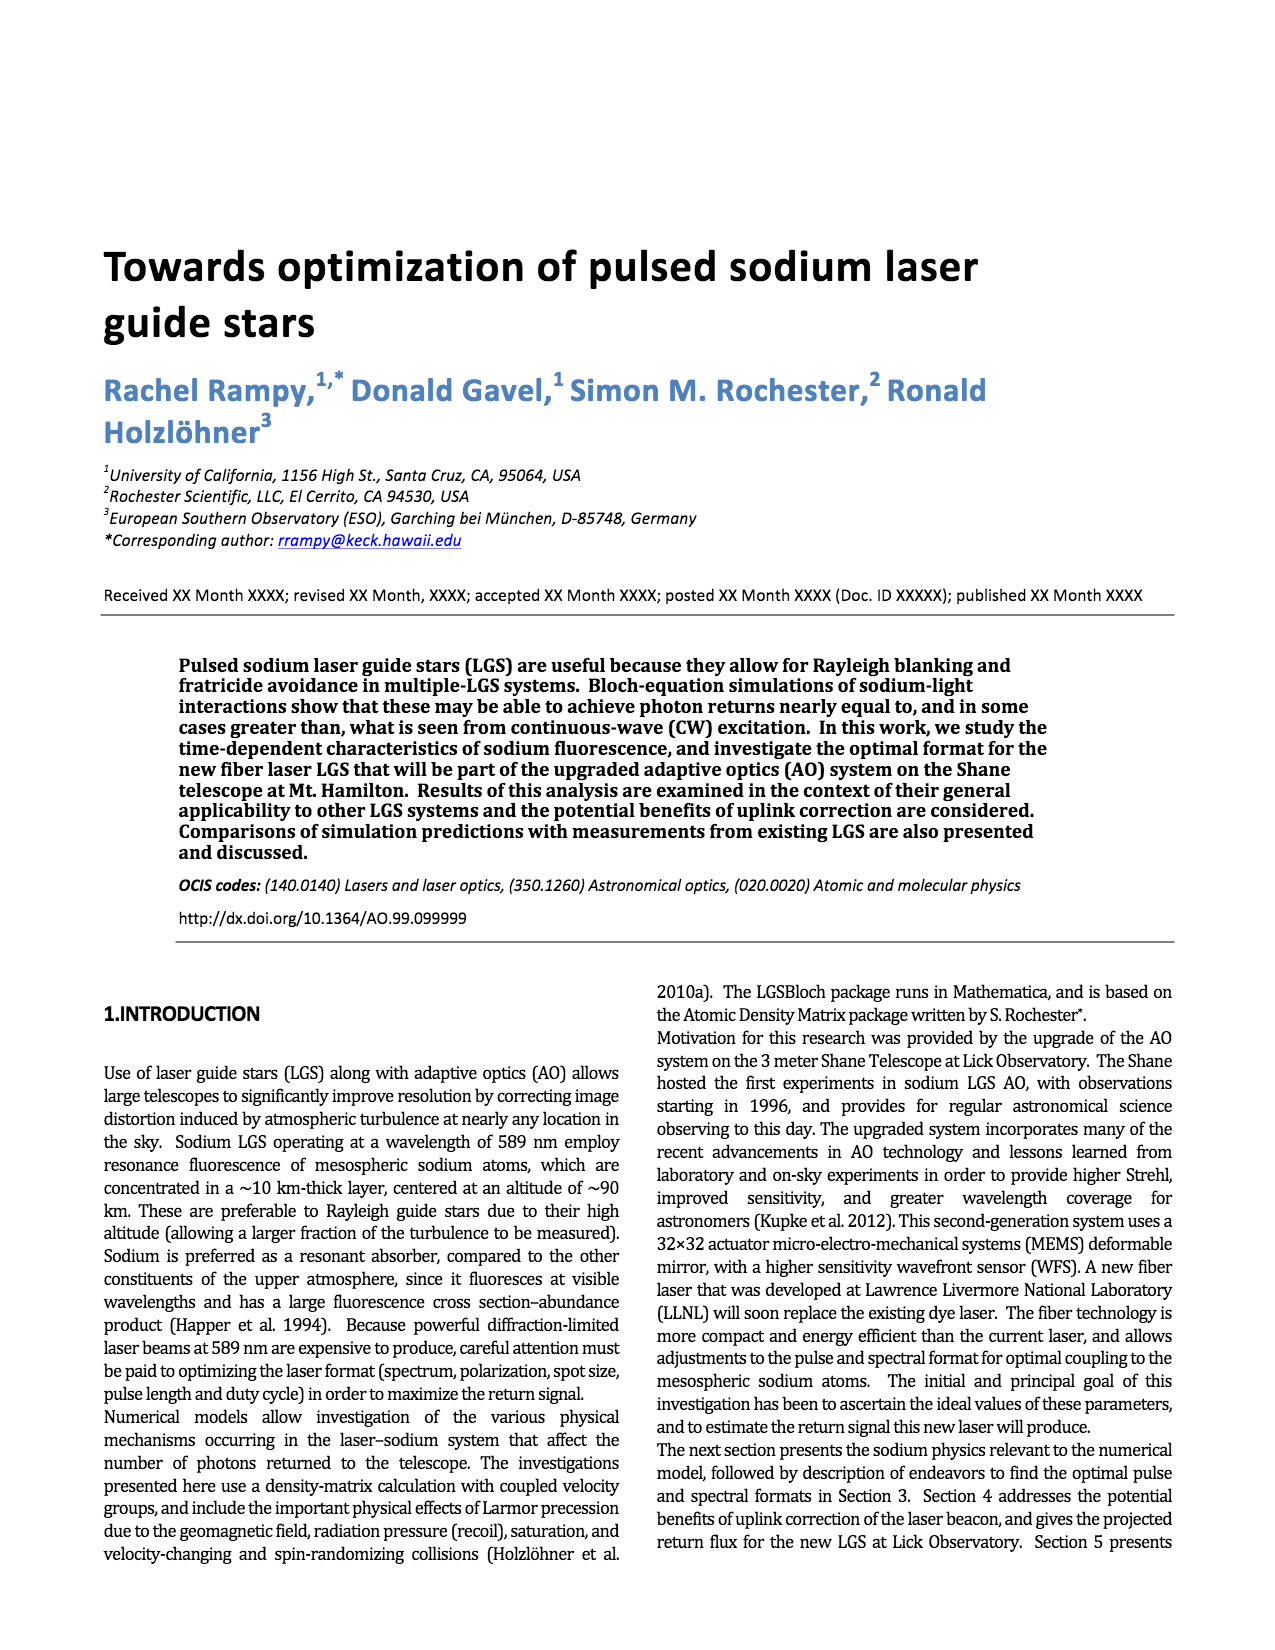
\includepdf[pages = -]{PDF/optimization_pulsed_lgs.pdf}

\section*{Holzlöhner, R., et al. "Optimization of cw sodium laser guide star efficiency." Astronomy \& Astrophysics 510, A20 (2010).}

I believe that this paper is a more in depth description of Rampy's paper. I think Rampy was an undergrad or grad student who wrote the above paper, and then possibly their advisor wrote a second edition or so?

%\includepdf[pages=-]{PDF/optimization_of_cw_lgs.pdf}

\section*{Sohl, John E., and Stephen G. Payton. "A modular, reconfigurable-cavity, pulsed dye laser for the advanced undergraduate laboratory." American Journal of Physics 65.7, 640-652 (1997).}

This is the paper that we used to make our first dye laser. It describes a very simple dye laser which can be make quite easily and cheaply. This may be the setup we use for our experiment.

\section*{ Watanabe, Makoto, et al. "Proceedings of SPIE-The International Society for Optical Engineering." Advancements in Adaptive Optics, (2004).}
A thorough paper on adaptive optics in real world systems. Quite extensive and not directly necessary for my paper.

Useful in explaining applications of my experiment

%\section*{Wizinowich, Peter L., David Le Mignant, Antonin H. Bouchez, Randy D. Campbell, Jason CY Chin, Adam R. Contos, Marcos A. van Dam et al. "The WM Keck Observatory laser guide star adaptive optics system: overview." Publications of the Astronomical Society of the Pacific 118, no. 840, 297 (2006).}



\end{document}
